%source mathadata
\begin{multicols}{2}
		\begin{MADenumerate}

			\item On considère les points $A(1;2)$ et $B(5;4)$. Dans la suite, on cherchera un premier point à égale distance d'eux placé sur le segment $[AB]$.
			\begin{enumerate}
				\item Placer les points $A$ et $B$ dans le repère. Placer le milieu $M$ de $[AB]$ et donner ses coordonnées par lecture graphique.
				\item Vérifier qu'on obtient le même résultat en calculant les moyennes des abscisses et des ordonnées de $A$ et $B$.
			\end{enumerate}

			\item Vérifier que le point $M$ est à égale distance de $A$ et de $B$ en calculant les distances $MA$ et $MB$.

			\item Calculer $AB$ et $MA + MB$. Que remarque-t-on ?

			\item L'égalité obtenue n'est-elle vraie que pour le milieu du segment $[AB]$ ?

			\item Écrire la formule générale des coordonnées du milieu dans l'encadré.

		\end{MADenumerate}

		\columnbreak

		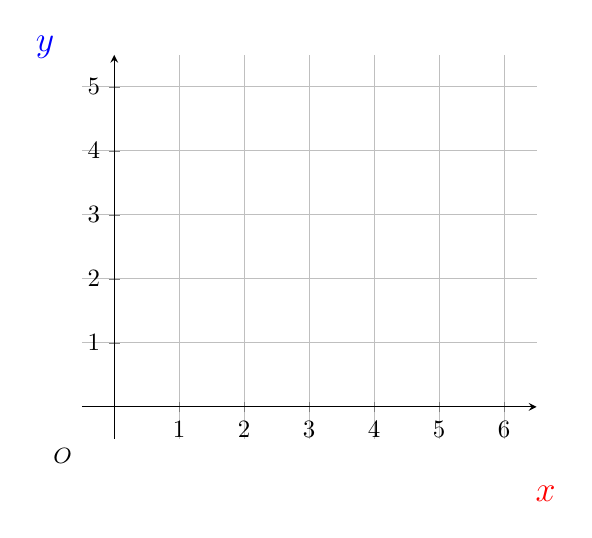
\begin{tikzpicture}[scale=0.9]
			\begin{axis}[
					name=plotM,
					axis lines=middle,
					ymajorgrids=true,
					xmajorgrids=true,
					xmin=-0.5,
					xmax=6.5,
					ymin=-0.5,
					ymax=5.5,
					xtick={0,1,...,6},
					ytick={0,1,...,5},
					xlabel={\Large{\color{red}$x$}},
					xlabel style={at={(axis description cs:1.02,-0.1)}, anchor=north},
					ylabel={\color{blue}{\Large$y$}},
					ylabel style={at={(axis description cs:-0.12,1.02)}, anchor=west},
					width=8cm,
					height=7cm,
				]
			\end{axis}
			\draw (0,0) node[below left]{\footnotesize $O$};
		\end{tikzpicture}
		\begin{bilan}[Point milieu d'un segment]
			Soient $A(x_A ; y_A)$ et $B(x_B;y_B)$ deux points quelconques. Le point milieu $M$ de $[AB]$ a pour coordonnées :
			$$M(\ligne[2cm] ; \ligne[2cm])$$
		\end{bilan}

	\end{multicols}
